\section{Đánh giá mô hình}
%\subsection{Confusion matrix}
\textbf{Confusion matrix} (ma trận nhầm lẫn hay ma trận lỗi) là một trong các kỹ thuật tính toán hiệu suất thường được sử dụng trong các bài toán phân loại.\\

Với bài toán đang xét gồm có 3 lớp thì ta có ma trận nhầm lẫn cho 3 lớp ví dụ như hình sau:
\begin{center}
    \begin{figure}[!h]
        \centering
        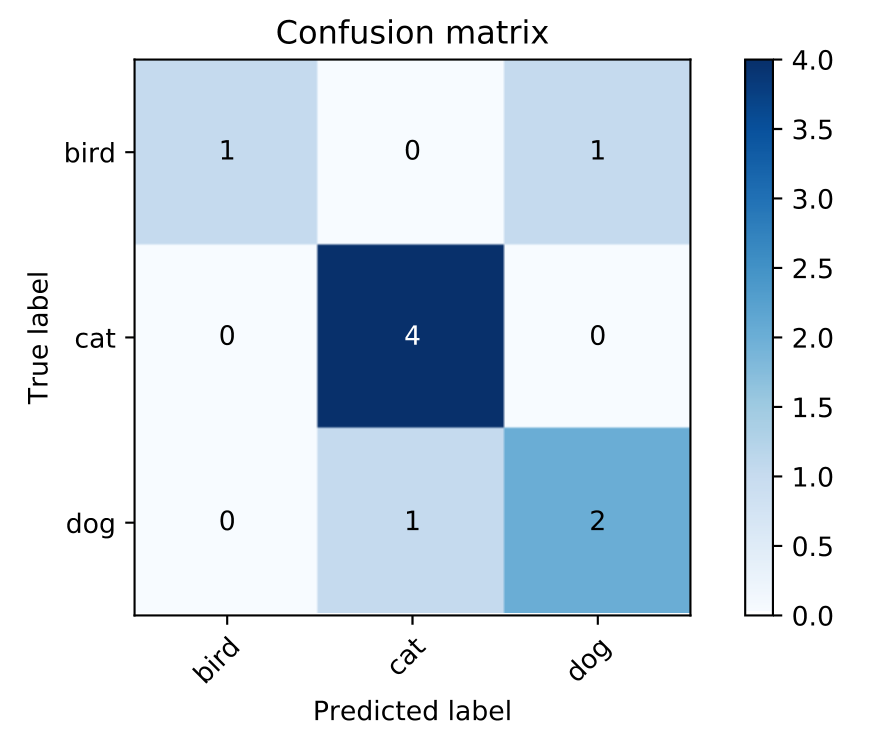
\includegraphics[scale = 0.5]{fileanh/6.png}
        \caption{confusion matrix}
    \end{figure}
\end{center}
Ví dụ ta xét lớp \textbf{Birt} thì True Positives (TP), False Positives (FP), False Negatives (FN) và True Negatives (TN) sẽ được xác định
\begin{center}
    \begin{figure}[!h]
        \centering
        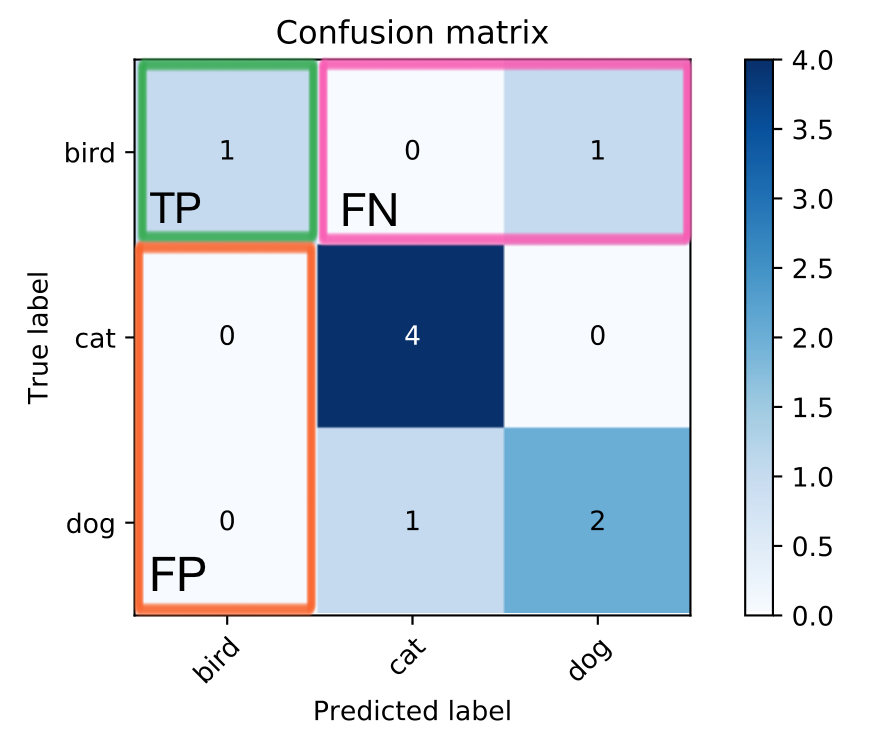
\includegraphics[scale = 0.5]{fileanh/7.png}
        \caption{Xác định TP, FP, FN cho lớp Birt}
    \end{figure}
\end{center}
True Negatives (TN) sẽ được hiểu các ô còn lại trong đó. Từ đây ta có:
\begin{itemize}
    \item True Positives (TP): là giá trị của ô vuông có tên của nhãn thực sự và nhãn dự đoán trùng nhau.
    \item False Positives (FP): là giá trị của 2 ô còn lại xét theo cột nhãn dự đoán của lớp cần tìm.
    \item False Negatives (FN): là giá trị của 2 ô còn lại xét theo cột nhãn thực sự của lớp cần tìm.
    \item True Negatives (TN): là giá trị của các ô còn lại.
\end{itemize}
Cuối cùng thu được bảng kết quả:
\begin{center}
    \begin{figure}[!h]
        \centering
        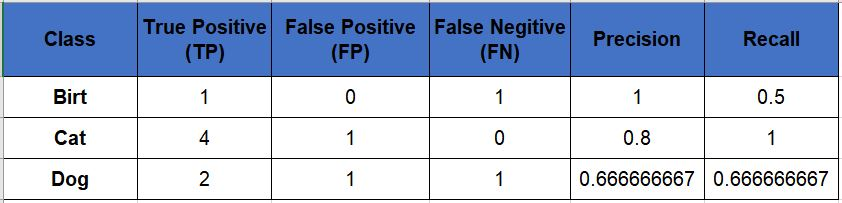
\includegraphics[scale = 1]{fileanh/8.jpg}
        \caption{Xác định TP, FP, FN cho lớp Birt}
    \end{figure}
\end{center}
Trong đó:
$\displaystyle \text{Precision}\ = \frac{TP}{TP + FP},\ \text{ Recall}\ = \frac{TP}{TP + FN}$\\

\textbf{Macro average precision} (Độ chính xác trung bình vĩ mô) là giá trị trung bình của tất cả các Precision của mỗi lớp.
$$\text{PrecisionMacroAvg}\ = \frac{Prec_1 + Prec_2 + \cdots + Prec_n}{n}$$
Xét ví dụ trên, có:
$$\text{PrecisionMacroAvg}\ = \frac{Prec_{Birt} + Prec_{Cat} + Prec_{Dog}}{3} = \frac{1 + 0.8+0.6667}{3} = 0.8222$$


\textbf{Macro average recall} (Khả năng thu hồi trung bình vĩ mô) là giá trị trung bình cộng của tất cả các Recall của mỗi lớp.
$$\text{RecallMacroAvg}\ = \frac{Recall_1 + Recall_2 + \cdots + Recall_n}{n}$$
Xét ví dụ trên, có:
$$\text{RecallMacroAvg}\ = \frac{Recall_{Birt} + Recall_{Cat} + Recall_{Dog}}{3} = \frac{0.5 + 1+0.6667}{3} = 0.7222$$


\textbf{F1-score} - điểm F cân bằng hay thước đo F có thể hiểu là trung bình điều hòa của độ chính xác (precision) và khả năng thu hồi (recall).
$$F_1 = \frac{2*(Precision * Recall)}{Precision + Recall}$$